\documentclass[11pt,]{article}
\usepackage{lmodern}
\usepackage{amssymb,amsmath}
\usepackage{ifxetex,ifluatex}
\usepackage{fixltx2e} % provides \textsubscript
\ifnum 0\ifxetex 1\fi\ifluatex 1\fi=0 % if pdftex
  \usepackage[T1]{fontenc}
  \usepackage[utf8]{inputenc}
\else % if luatex or xelatex
  \ifxetex
    \usepackage{mathspec}
  \else
    \usepackage{fontspec}
  \fi
  \defaultfontfeatures{Ligatures=TeX,Scale=MatchLowercase}
    \setmainfont[]{Arial}
\fi
% use upquote if available, for straight quotes in verbatim environments
\IfFileExists{upquote.sty}{\usepackage{upquote}}{}
% use microtype if available
\IfFileExists{microtype.sty}{%
\usepackage{microtype}
\UseMicrotypeSet[protrusion]{basicmath} % disable protrusion for tt fonts
}{}
\usepackage[margin=.5in]{geometry}
\usepackage{hyperref}
\hypersetup{unicode=true,
            pdfborder={0 0 0},
            breaklinks=true}
\urlstyle{same}  % don't use monospace font for urls
\usepackage{natbib}
\bibliographystyle{plainnat}
\setlength{\emergencystretch}{3em}  % prevent overfull lines
\providecommand{\tightlist}{%
  \setlength{\itemsep}{0pt}\setlength{\parskip}{0pt}}
\setcounter{secnumdepth}{5}

%%% Use protect on footnotes to avoid problems with footnotes in titles
\let\rmarkdownfootnote\footnote%
\def\footnote{\protect\rmarkdownfootnote}


  \title{}
    \author{}
    \date{}
  

%%%%%%%%%%
% personal preamble edits here
%%%%%%%%%%
\pagenumbering{gobble}

% can toggle this for Helvetica
%\usepackage{helvet}
%\renewcommand{\familydefault}{\sfdefault}

% \titlespacing*{\paragraph}{0pt}{2pt}{1em}

% set section numbering/lettering
% tips for seccntformat: https://tex.stackexchange.com/questions/95896/how-to-format-subsection-title-without-packages
\makeatletter
\def\@seccntformat#1{%
  \expandafter\ifx\csname c@#1\endcsname\c@section\else
  \expandafter\ifx\csname c@#1\endcsname\c@paragraph\else
  \csname the#1\endcsname\quad
  \fi\fi}
  
  % stucture for these commands: https://texfaq.org/FAQ-atsigns
  \renewcommand\section{
  \@startsection{section}{1}{\z@}
    {-3.5ex \@plus -1ex \@minus -.2ex}
    {1.0ex \@plus.2ex} %reduce space below section (was 1.5ex)
    {\normalfont\normalsize\bf\uppercase}} %modify font style
    
  \renewcommand\subsection{
  \@startsection{subsection}{2}{\z@}
    {-1.5ex\@plus -1ex \@minus -.2ex}%reduce space above subsection (was -3.25ex)
    {0.5ex \@plus .2ex}%reduce space below subsection (was 1.5ex)
    {\normalfont\normalsize\bf}} %modify font style
    
  \renewcommand\subsubsection{
  \@startsection{subsubsection}{3}{\z@}
    {-1.0ex\@plus -1ex \@minus -.2ex}%reduce space above subsubsection (was -3.25ex)
    {0.5ex \@plus .2ex}%reduce space below subsubsection (was 1.5ex)
    {\normalfont\normalsize\bf}} %modify font style
    
  \renewcommand\paragraph{
  \@startsection{paragraph}{4}{\z@}
    {-0.5ex\@plus -1ex \@minus -.2ex}%reduce space above paragraph (was -3.25ex)
    {-1.5ex \@plus .2ex}%convert space below paragraph to an indent (was 1.5ex)
    {\normalfont\normalsize\bf}} %modify font style    
\makeatother

\renewcommand\thesubsection{\Alph{subsection}.}
\renewcommand\thesubsubsection{\thesubsection\arabic{subsubsection}.}

% reduce spacing at the top of lists
\usepackage{enumitem}
\setlist{topsep = 2pt}

% allow text to wrap around figures
\usepackage{graphicx}
\usepackage{wrapfig}

%%%%%%%%%%

\begin{document}

\hypertarget{project-summaryabstract}{%
\section{Project Summary/Abstract}\label{project-summaryabstract}}

Do this last.

\pagebreak

\hypertarget{specfic-aims}{%
\section{Specfic Aims}\label{specfic-aims}}

At the highest level, what is the area the study focuses on?

What have I done that is relevant to the study?

What are the hypotheses the initial work has generated, which will be
the focus of the study.

Specific Aims: title what is going to be done

What comes next? What will the impact be of achieving the specific aims?

\hypertarget{research-strategy}{%
\section{Research Strategy}\label{research-strategy}}

\hypertarget{significance}{%
\subsection{Significance}\label{significance}}

Reintroduce the domain.

What is the impact/significance of what is done now?

What does the study do?

How will this change research in the domain?

\hypertarget{important-significance-topic.}{%
\paragraph{Important significance
topic.}\label{important-significance-topic.}}

\hypertarget{another-important-significance-topic.}{%
\paragraph{Another important significance
topic.}\label{another-important-significance-topic.}}

\hypertarget{innovation}{%
\subsection{Innovation}\label{innovation}}

What is different/new/novel about this project?

\begin{itemize}
\tightlist
\item
  Some bullets may be helpful to the reviewers here.
\item
  Some bullets may be helpful to the reviewers here too.
\end{itemize}

\hypertarget{approach}{%
\subsection{Approach}\label{approach}}

Background - what are the existing concepts this study will use? How
will they be put together?

\hypertarget{specific-aim-title}{%
\subsection{Specific Aim: Title}\label{specific-aim-title}}

Hypothesis: What is being tested? Rationale: Why is this something we
should be testing? Experimental Approach: How is the test going to be
implemented? Interpretation of Results: How does the test translate to
science? Potential Problems and Alternative Approaches: What will we do
if it doesn't work?

Note: Material below is for reference.

\hypertarget{overview-of-the-proposal}{%
\subsubsection{Overview of the
proposal}\label{overview-of-the-proposal}}

\hypertarget{research-team}{%
\subsubsection{Research team}\label{research-team}}

\hypertarget{preliminary-studies}{%
\subsubsection{Preliminary studies}\label{preliminary-studies}}

\begin{wrapfigure}{R}{0.3\textwidth}

\hfill{}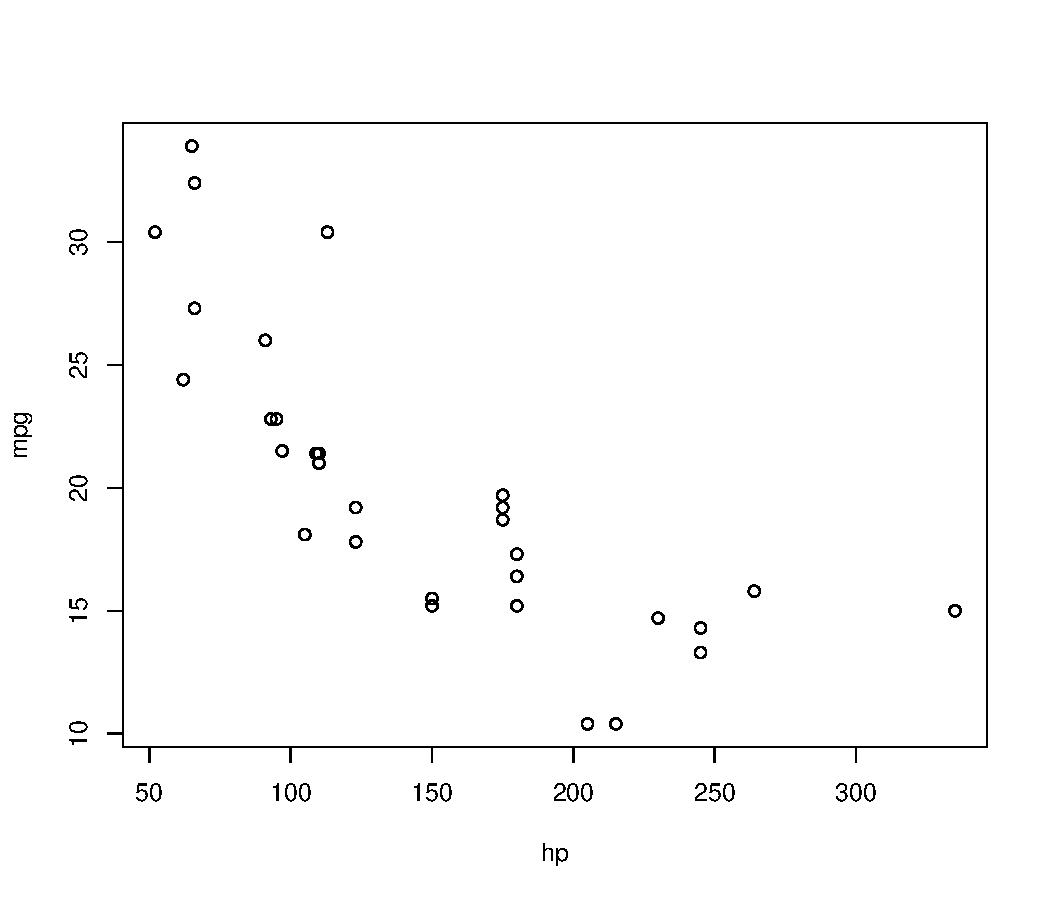
\includegraphics[width=.3\textwidth]{Project-Proposal_files/figure-latex/unnamed-chunk-2-1} 

\caption{Important scatterplot}\label{fig:unnamed-chunk-2}
\end{wrapfigure}

\hypertarget{resources}{%
\subsubsection{Resources}\label{resources}}

\hypertarget{design-and-methods-for-aim-1}{%
\subsubsection{Design and methods for Aim
1}\label{design-and-methods-for-aim-1}}

\hypertarget{design-and-methods-for-aim-2}{%
\subsubsection{Design and methods for Aim
2}\label{design-and-methods-for-aim-2}}

\hypertarget{design-and-methods-for-aim-3}{%
\subsubsection{Design and methods for Aim
3}\label{design-and-methods-for-aim-3}}

\hypertarget{timeline}{%
\subsubsection{Timeline}\label{timeline}}

There are lots of good examples of \texttt{R}-based Gantt charts to be
found by clever Googling. For displaying progress with sidebar
annotations by aim, I particularly like
\href{https://datascienceplus.com/visualize-your-cvs-timeline-with-r-gantt-style/}{\underline{this}}
example from the
\href{https://github.com/laresbernardo/lares}{\underline{lares}}
package.

\hypertarget{rigor-and-reproducibility}{%
\subsubsection{Rigor and
reproducibility}\label{rigor-and-reproducibility}}

\hypertarget{impact-of-the-proposed-study}{%
\subsubsection{Impact of the proposed
study}\label{impact-of-the-proposed-study}}

\bibliography{references.bib}


\end{document}
